\documentclass{beamer}
\usepackage{amsmath}
\usepackage{amsfonts}
\usepackage{amssymb}
\usepackage{verbatim}
\usepackage{graphicx}
\usepackage{subfig}

\usetheme{Rochester}
%\usefonttheme[onlymath]{serif}
%\setbeamertemplate{caption}[numbered]
%\setbeamertemplate{enumerate items}[default]

\title{ Boundary Effects in Stochastic Cyclic Competition Models on a Two-Dimensional Lattice}
\author{M. Lazarus Arnau, Shannon Serrao, Uwe C. T\"auber}
\institute
{
    Department of Physics,\\
    Virginia Polytechnic Institute and State University
}
\date{March 7, 2019 \\
        \begin{figure}[t]
            \centering
            
\includegraphics[width=0.15\linewidth]{images/aro_logo_t.png}
            \label{fig:aro_logo_t}
        \end{figure}
}

\begin{document}

    \frame{\titlepage}

    \begin{frame}[t]{Typical Behavior}
        \begin{figure}[h]
            \centering
            \subfloat[ $ \epsilon_r = 1.25 $ ]{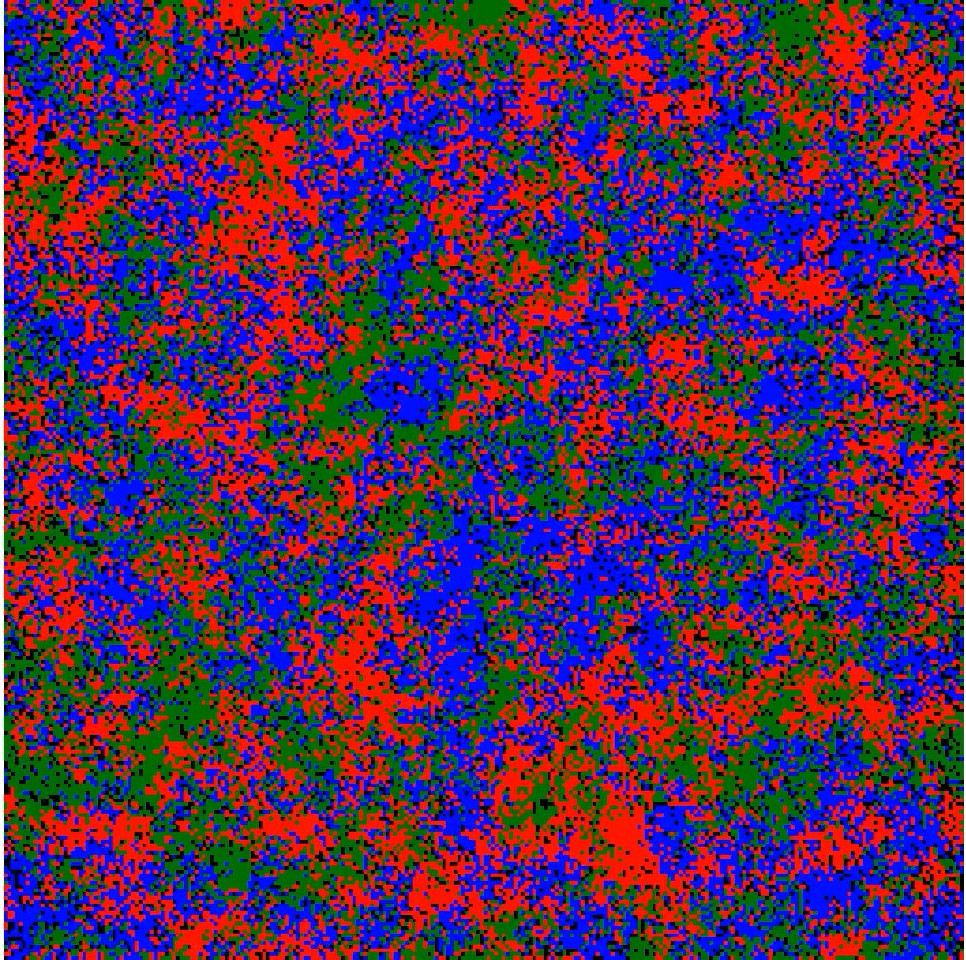
\includegraphics[width=0.4\linewidth]{images/rps_1_25.jpg}}
            \subfloat[ $ \epsilon_m = 5.0 $ ]{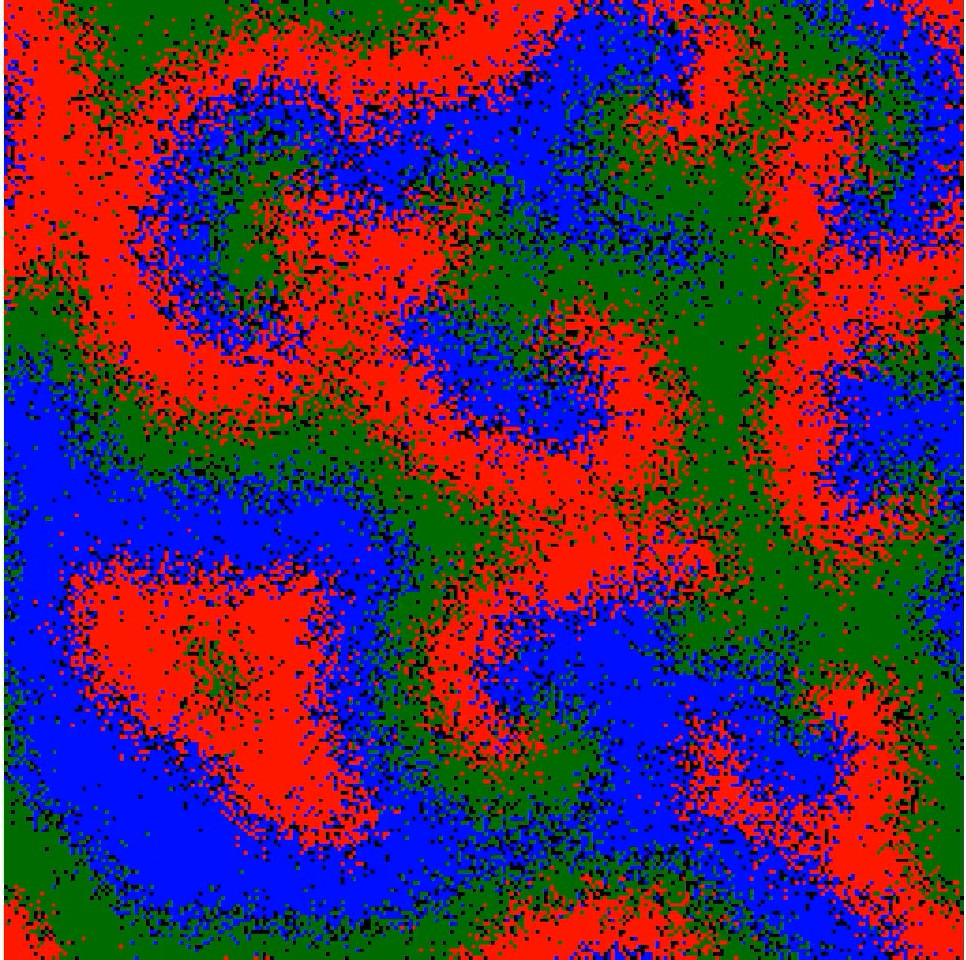
\includegraphics[width=0.4\linewidth]{images/ml_5_0.jpg}}
            \caption{Typical steady state snapshots of Rock-Paper-Scissors (a) and May-Leonard (b) systems }
            \label{fig:name}
        \end{figure}
    \end{frame}
    \begin{frame}
        \frametitle{Models}

        Three species cyclic competition schemes motivated by examples in biology, population dynamics, and chemistry.
                
        \begin{itemize}
            \item Rock-Paper-Scissors (RPS) Model
                \begin{align*}
                    (\text{Replacement}) & X_nX_{n+1} \xrightarrow{\zeta} X_n X_n\\
                    (\text{Hopping}) & XY \xrightarrow{\epsilon_r} YX \\
                \end{align*}

            \item May-Leonard (ML) Model
                \begin{align*}
                    (\text{Predation}) & X_nX_{n+1} \xrightarrow{\sigma} X_n \varnothing \\
                    (\text{Reproduction}) & X \varnothing \xrightarrow{\mu} XX \\
                    (\text{Hopping}) & XY \xrightarrow{\epsilon_m} YX \\
                \end{align*}

                $ n $ represents the species index where $ X_4 = X_1 $ 
        \end{itemize}
    \end{frame}


    \begin{frame}
        \frametitle{Combined System}
        \begin{figure}[h]
            \centering
            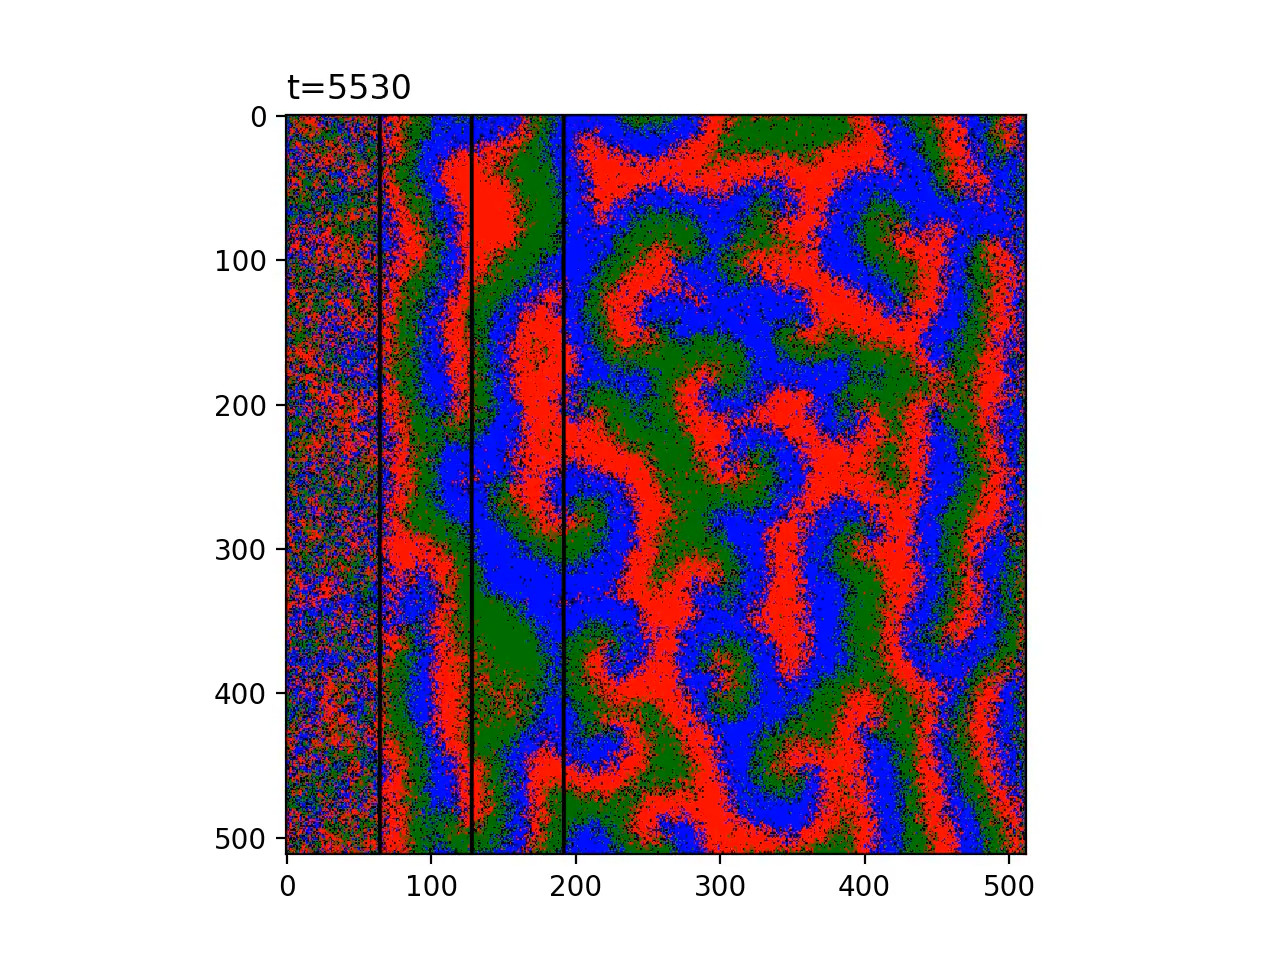
\includegraphics[width=0.75\linewidth]{images/plane_wave_2.jpg}
            \caption{Plane wave formation }
            \label{fig:plane_wave_2}
        \end{figure}
    \end{frame}

    \begin{frame}[t]{Correlation Lengths and Permeation Distance}
        \begin{figure}[h]
            \centering
            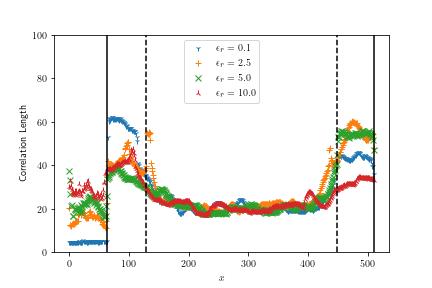
\includegraphics[width=0.75\linewidth]{images/correlation_lengths.png}
            \caption{Correlation length}
            \label{fig:correlation_length}
        \end{figure}
        
    \end{frame}

    \begin{frame}[t]{Well-Mixing Effects}
        \framesubtitle{Boundary Effects}
        \begin{figure}[h]
            \centering
            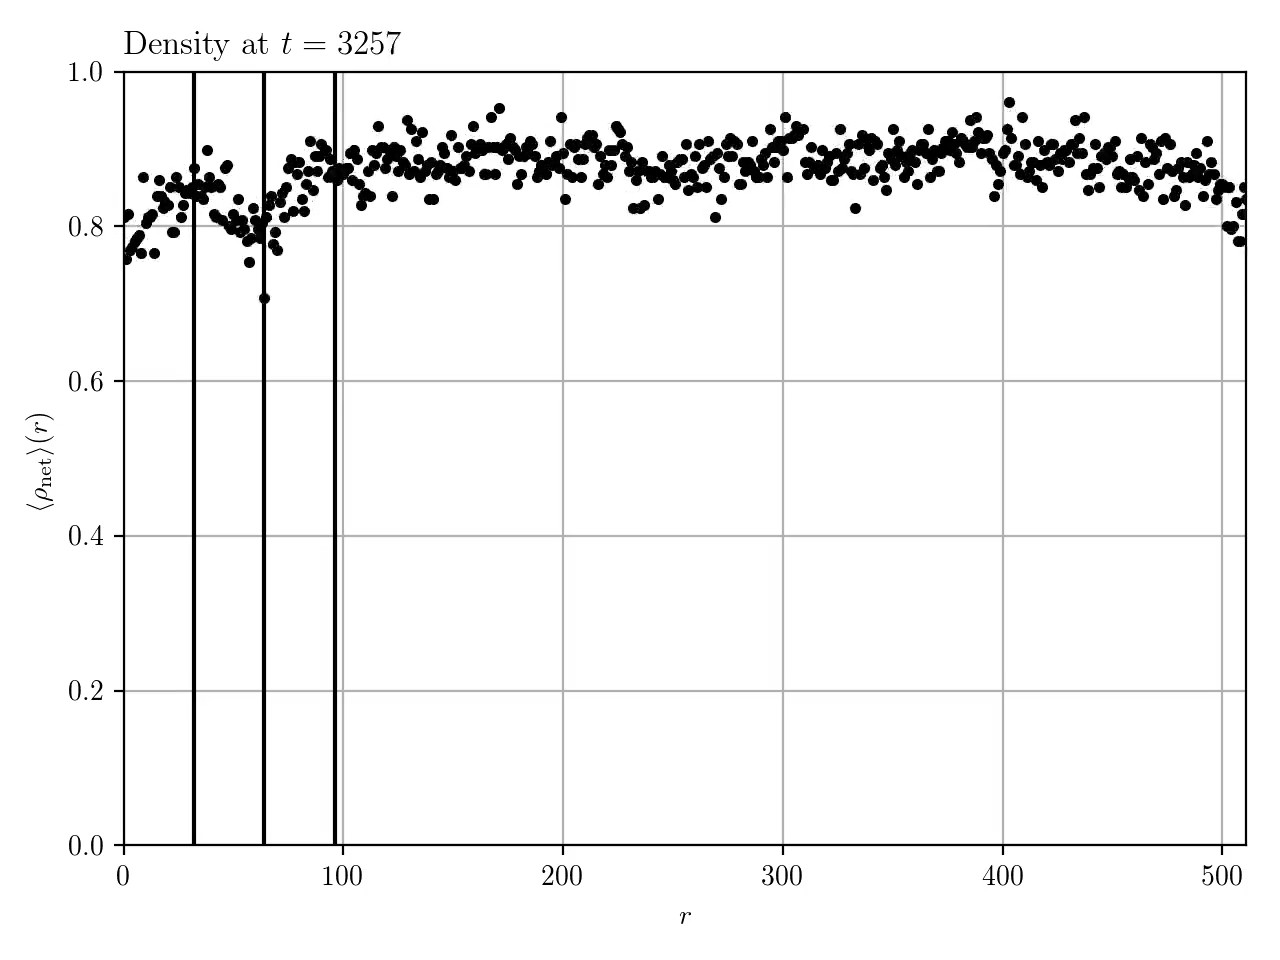
\includegraphics[width=0.75\linewidth]{images/net_density_2_5.jpg}
            \caption{Prominent drop in net population density}
            \label{fig:mixing}
        \end{figure}
    \end{frame}

    \begin{frame}[t]{Well-Mixing Effects}
        \framesubtitle{Boundary Effects cont.}
        \begin{figure}[h]
            \centering
            {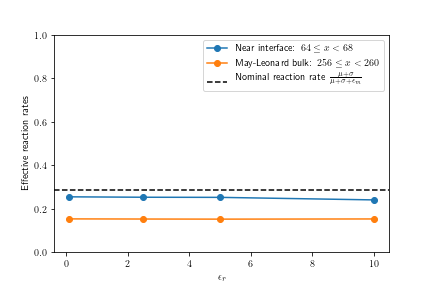
\includegraphics[width=0.9\linewidth]{images/reaction_rates.png}}
            \caption{ Relative reproduction $+$ predation rates near the boundary 
            vs. in May-Leonard bulk}
            \label{fig:mixing}
        \end{figure}
    \end{frame}

    \begin{frame}[t]{Well-Mixing Effects}
        \framesubtitle{Transient Effects}

        \begin{figure}[h]
            \centering
            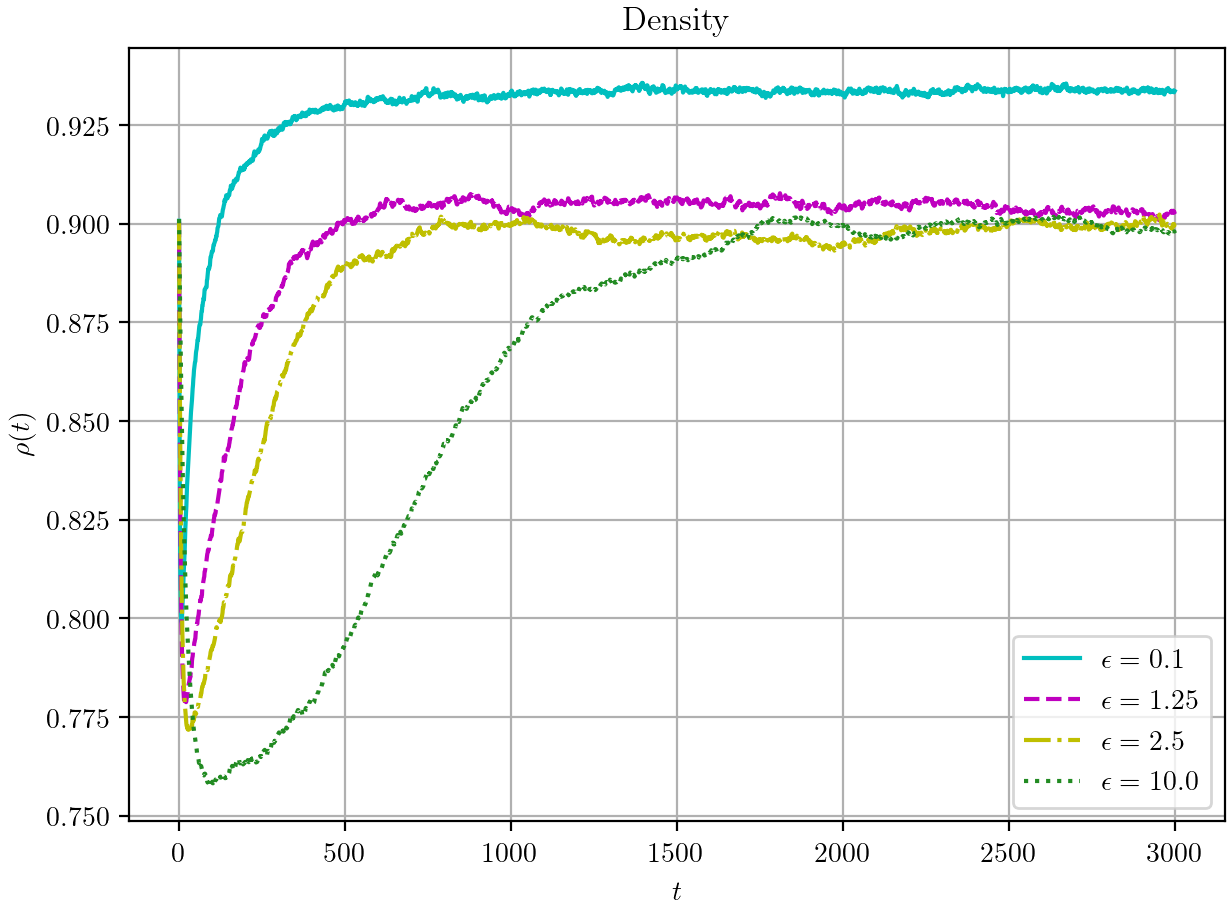
\includegraphics[width=0.7\linewidth]{images/densities_try_0.png}
            \caption{ From random initial conditions ML model approaches mean-field density before
            relaxing to steady state.}
            \label{fig:images/densities_try_0}
        \end{figure}
    \end{frame}

    \begin{frame}[t]{Conclusions and questions}
        \begin{itemize}
            \item Competion between different models can influence their long term behaviors.

            \item Disruptions in pattern formation caused by "mixing" of particles
                  the boundary.

        \end{itemize}

        \begin{figure}[t]
            \centering
            
\includegraphics[width=0.2\linewidth]{images/aro_logo_t.png}
            \label{fig:aro_logo_t}
        \end{figure}
    \end{frame}
\end{document}

